\documentclass{article}

\usepackage{ext/arxiv}

\usepackage[utf8]{inputenc} % allow utf-8 input
\usepackage[T1]{fontenc}    % use 8-bit T1 fonts
\usepackage{hyperref}       % hyperlinks
\usepackage{url}            % simple URL typesetting
\usepackage{booktabs}       % professional-quality tables
\usepackage{amsfonts}       % blackboard math symbols
\usepackage{nicefrac}       % compact symbols for 1/2, etc.
\usepackage{microtype}      % microtypography
\usepackage{cleveref}       % smart cross-referencing
\usepackage{graphicx}
\usepackage{natbib}
\usepackage{subcaption}
\usepackage{doi}

\title{Barnyard Karaoke: Recreating Melodies with Animal Sounds}

% Here you can change the date presented in the paper title
%\date{September 9, 1985}
% Or remove it
\date{}

\author{
	Patricio Ovalle \\
	Universitat Pompeu Fabra\\
	Barcelona, Spain \\
	\texttt{patricio.ovalle01@estudiant.upf.edu}
}

%%% Add PDF metadata to help others organize their library
%%% Once the PDF is generated, you can check the metadata with
%%% $ pdfinfo template.pdf
\hypersetup{
pdftitle={Barnyard Karaoke: Recreating Popular Melodies with Animal Sounds},
pdfauthor={Patricio Ovalle},
pdfkeywords={Audio, Mosaicing, Animal, Sounds},
}

\begin{document}
\maketitle



\section{Introduction}

Audio mosaicing refers to the technique of reconstructing a target audio using only material from a collection of source audio.
This project explores using audio mosaicing as a means to orchestrate new arrangements of popular melodies using animal sounds.
The goal is to produce audio that evokes a medley of barn animals howling in the yard for a carefree evening of karaoke.

The idea takes inspiration from \textit{Meowify}\footnote{https://github.com/gulnazaki/meowify}, a project that replaces singing voice with cats meowing.
Their method consists of two steps: first, a source separation model is used to isolate the vocals from the rest of the mix; then, a timbre transfer model is used to morph the singing voice into a cat's meow before recombining the modified vocals with the rest of the mix.
This project attempts to achieve a similar result via the technique of audio mosaicing.
The code for this project is openly available online\footnote{https://github.com/p3zo/barnyard-karaoke}.

\section{Methodology}

Audio mosaicing consists of two distinct components: a target audio and a set of source audio.
To decide how the source audio should be split and recombined to reconstruct the target, several key decisions must be made:

\begin{itemize}
  \item the characteristics to emulate in a target sound
  \item the selection of a target sound
  \item the selection of a set of source audio
  \item a method for selecting source audio frames
  \item a method for recombining selected frames
\end{itemize}

The following sections address each of these concerns and describe the strategies used at each step.

\subsection{Target characteristics}

The first step to define the characteristics of the target sound we want to preserve.
Our aim is to reconstruct a melody, so the pitches and pitch onset times of the melody in the target audio are the most essential features to extract.

To analyze the pitch contour of the predominant melody from the audio, we use the MELODIA algorithm introduced by \citet{salamon2012melody} and implemented in the Essentia audio analysis toolkit \citep{bogdanov2013essentia}.
To subsequently determine the pitch onset times of the melody, we use the pitch contour segmentation algorithm in Essentia introduced by \citet{mcnab1995signal}.
This segmentation algorithm is especially convenient for our needs as it takes a pitch contour as input, which is the output of the MELODIA algorithm.
A downside of this algorithm is that it requires a fine-tuning of several parameters in order to function well.
For its "hopSize" and "minDuration" parameters we choose relatively small values to ensure it captures the rhythmic nuance of the melodies.
Specifically, we derive the minimum note duration using the tempo of the target tracks together with the shortest note values used in their melodies.
For a track at 90 beats per minute (bpm), the duration in seconds for an eighth note is given by: \[\frac{60\ seconds}{90\ bpm} * \frac{1}{2}\ beat = .33\ seconds\]
For each track we set the "minDuration" parameter to just below this value to account for some variation in tempo.
We set the "rmsThreshold" parameter to be low as well because we deem over-detecting onsets to be better than under-detecting them for this application.
The result of extraneous onsets is that more than one source frame will be used to reconstruct a given melodic pitch in the target.
On the other hand the result of a missing onset is silence, which makes for a less exciting output.
An example of an estimated pitch contour and its detected onsets are shown in Figures~\ref{pitch-contour} and \ref{onsets}.

\begin{figure}[ht]
    \begin{center}
        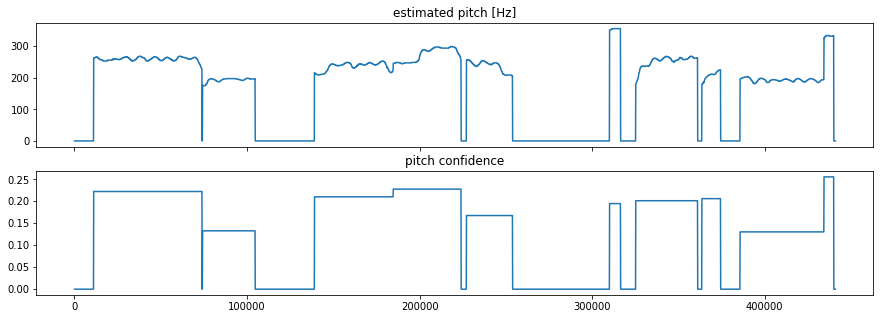
\includegraphics[width=0.7\textwidth]{pitch-countour}
    \end{center}
    \caption{A pitch contour estimated using MELODIA}
    \label{pitch-contour}
\end{figure}

\begin{figure}[ht]
    \begin{center}
        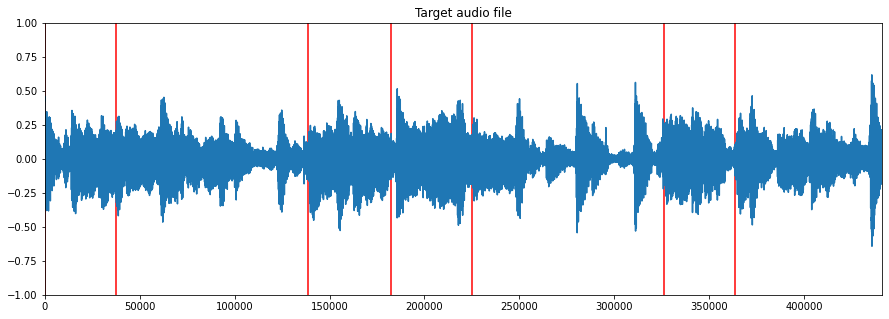
\includegraphics[width=0.7\textwidth]{onsets}
    \end{center}
    \caption{Original audio with estimated pitch onset time markers}
    \label{onsets}
\end{figure}

\subsection{Target sound selection}

The next concern is to select the target sound for which we want to emulate the pitch contours. Our aim is to recreate melodies, so we choose musical tracks with well-known melodies as targets. In particular, we choose two tracks with simple vocal melodies that are easy to sing along to. The tracks are listed in Table~\ref{tab:target-songs} along with the timestamps used from each.

An important consideration is to select a sound with not too much complexity in the mixture to increase the effectiveness of a general pitch-tracking algorithm for melody extraction. We selected only target sounds in which the melodies were predominant and in a distinct pitch range from other instruments in the arrangement.


% TABLE: TARGET SOUNDS
\begin{table}
    \begin{center}
    \begin{tabular}{@{}lll@{}}
        \toprule
        Youtube ID & Title & Timestamp \\
        \midrule
        V1bFr2SWP1I & Somewhere Over the Rainbow & 1:05 - 1:15 \\
        \_6HzoUcx3eo & Old Macdonald Had A Farm & 0:15 - 0:35 \\
        \bottomrule
    \end{tabular}
    \end{center}
    \caption{Target songs}
    \label{tab:target-songs}
\end{table}



\subsection{Source sound collection}

The source collection in audio mosaicing is the set of audio from which frames can be sliced and used as material to recreate the melody of the target.
Our aim is to create a set of animal sounds that are well-pitched and clearly recognizable.

We download our collection of audio samples from Freesound\footnote{https://freesound.org} using their API.
The parameters used in the Freesound API queries are shown in Table~\ref{tab:source-collection-queries}.
We select a set of animals that produce sounds in different registers overlapping with the range of the human voice.
We also select animals with distinct timbres from one another in hopes of adding a bit of dynamism to the result.
Each API query included a sort condition by descending user rating to get the highest-rated sounds first.
In a manual exploration of downloaded results we noticed that shorter recordings were typically of higher quality than longer recordings, which often tended to be field recordings clouded with background noise and various non-animal sounds.
Each collection was filtered to a short duration in order to increase the chance that the query would return single-shot sounds.
The moos and bleats were allowed to be slightly longer because it seems that cows and sheep take longer to vocalize their thoughts.

For comparison, we also create a second source collection of tuned, harmonic sounds.
Specifically, we download a set of violin notes from Freesound using the "ac\_single\_event" query parameter to specify that the audio should contain a single event, i.e. a single note played on the violin.


\subsection{Frame selection strategy}

When selecting which frames to use from the source to recreate the desired characteristics of the target audio, a similarity score is computed between each frame in the target audio and all of the frames in the source sound collection.
Among the top 10 highest scoring source frames, we choose one randomly so as to add a bit more variation in the result.

We experimented with several sets of features for computing this similarity, namely:

\begin{itemize}
  \item Pitch
  \item Pitch, loudness
  \item Pitch, loudness, and MFCCs
\end{itemize}

As previously mentioned, the pitch values were estimated from the MELODIA algorithm in Essentia.
The loudness and MFCC features were extracted using built-in algorithms in Essentia.
The goal with including loudness was to mimic the energy of the target melody, and the intent of using MFCC features was to capture the timbre of the instrument playing the melody.
We computed similarity with and without MFCCs with the expectation that timbre would be less important than pitch in producing a convincing result.
We also experimented with using pitch alone to see if omitting the other features would improve the general accuracy of pitch matching.


\subsection{Recombination strategy}

The final step in the audio mosaicing process is to define a strategy for how the selected source frames will be combined to reconstruct the target audio. We choose to recombine the selected frames at the pitch onset times determined by the segmentation algorithm. We elect to not allow the overlapping of source frames during recombination.

\section{Results}

Demos of both the animal and violin melody reconstructions can be heard at:
	\begin{center}
		\url{https://github.com/p3zo/barnyard-karaoke/tree/main/demo}.
	\end{center}

% TABLE: SOUND COLLECTION QUERIES
\begin{table}
    \begin{center}
    \begin{tabular}{@{}lll@{}}
        \toprule
        Count & Keyword & Max duration (seconds) \\
        \midrule
        5 & horse whinny &  5 \\
        5 & horse neighing &  5 \\
        10 & cat meow &  5 \\
        20 & dog bark &  1 \\
        20 & bleat &  10 \\
        20 & cow moo &  10 \\
        20 & bird chirp &  10 \\
        \bottomrule
    \end{tabular}
    \end{center}
    \caption{Query parameters used in Freesound API requests}
    \label{tab:source-collection-queries}
\end{table}

\section{Discussion}

Overall, the methodology described in this paper has a ways to go to produce the animal symphonies originally envisioned. The biggest improvement may come from assembling a well-curated sound collection. One glaring issue in the current animal sound collection is that many of the returned query results are actually sounds that are orthogonal to the query. For example, the query for "cat meow" returns results including the sound of pouring food in a cat bowl. Manual verification of the source sounds to remove non-animal sounds could go a long way. Additionally, there is a high degree of variability in the audio quality of the downloaded sounds. It would be helpful to have a few attributes related to audio quality to filter on when querying Freesound. For example a "signal-to-noise ratio" attribute would help filter out sounds with a lot of background noise. A "harmonic" attribute would be helpful in determining whether a sound is suitable to be used to match any pitch.

Another major improvement could come by using octave reduction. Some source frames match pitches in the target melodies but in a different octave. Labeling each source frame with its pitch class rather than its frequency would increase the coverage of pitch classes that can be matched exactly.

While the pitch detection algorithm used worked well on the selected target sounds, there are many complex mixtures for which it does not work well. For these cases, a source separation pre-processing step can be used to isolate the instrument playing the predominant melody, so as to simplify the input for pitch detection.


\bibliographystyle{unsrtnat}
\bibliography{main}

\end{document}
